\part{Non-linear equations II - Towards multi-dimensional case}
\section{Python solvers}
\begin{frame}[label=contents_integration]
  \frametitle{Today's outline}
  \mode<beamer>{
    \only<1>{\tableofcontents}
  }
  \only<2>{\tableofcontents[currentsection,currentsubsection]}
\end{frame}
\begin{frame}[fragile]
  \frametitle{Non-linear Equation Solving in Python (1 var)}

  \textbf{Single Variable Non-linear Zero Finding:}
  \begin{itemize}
      \item Use the \texttt{root\_scalar} function from \texttt{scipy.optimize} for finding zeros of a single-variable non-linear function.
      \item Be aware of the initial bracketing steps in \texttt{root\_scalar}.
  \end{itemize}

  \begin{lstlisting}[language=Python]
from scipy.optimize import root_scalar

root_scalar(lambda x: -3*x**2 - 5*x + 2, method='brentq', bracket=[1, 4], xtol=1e-15)
  \end{lstlisting}
  \lstinputlisting[style=PyOutput]{scripts/nonlinear/output_root_scalar.txt}
\end{frame}


\begin{frame}[fragile]
  \frametitle{Non-linear equation solver in Python ($\geq$ 2 var)}

  \textbf{Solving Systems of Non-linear Equations (Multiple Variables):}
  \begin{itemize}
      \item Use \texttt{fsolve} from \texttt{scipy.optimize} for systems involving multiple variables.
      \item Suitable for non-linear equations with two or more variables.
  \end{itemize}
  \begin{lstlisting}[language=Python]
from scipy.optimize import fsolve

def equations(x):
    return [2*x[0]*x[1] - x[1] + 2, 2*x[1] - 4*x[0] - 4]

fsolve(equations, [1, 1], xtol=1e-15)
    \end{lstlisting}
\end{frame}

\section{Newton-Raphson method}
\begin{frame}[fragile]
    \frametitle{Newton-Raphson Method}

    \textbf{Algorithm:}
    \begin{itemize}
        \item Requires evaluating both the function \( f(x) \) and its derivative \( f'(x) \) at arbitrary points.
        \item Extend the tangent line at the current point \( x_i \) until it intersects with zero.
        \item Set the next guess \( x_{i+1} \) as the abscissa of that zero crossing.
        \item For small enough \( \delta x \) and well-behaved functions, non-linear terms in the Taylor series become unimportant.
    \end{itemize}
    \vspace{-0.10cm}
    \begin{align*}
    f(x) &\approx f(x_i) + f'(x_i)\delta x + \mathcal{O}(\delta x^2) + \dots \\
    0 &\approx f(x_i) + f'(x_i)\delta x \\
    \delta x &\approx -\frac{f(x_i)}{f^\prime (x_i)} \\
    \end{align*}

    \vspace{-1.2cm}
    \begin{columns}
      \column{0.3\textwidth}
    \[
      \boxed{x_{i+1} = x_i - \frac{f(x_i)}{f'(x_i)}}
      \]   
    \column{0.6\textwidth}
    \begin{itemize}
        \item Can be extended to higher dimensions.
        \item Requires an initial guess close enough to the root to avoid failure.
    \end{itemize}
  \end{columns}
    
\end{frame}

\begin{frame}[fragile]
    \frametitle{Newton-Raphson Method}
    \vspace{-0.4cm}
    \begin{columns}
    \column{0.54\textwidth}
    \textbf{Example with the Formula:}
      \[
      x_{n+1} = x_n - \frac{f(x_n)}{f'(x_n)}
      \]
    \textbf{When it works:}
    \begin{itemize}
        \item Converges enormously fast when it functions correctly.
    \end{itemize}
    
    \textbf{When it does not work:}
    \begin{itemize}
        \item Underrelaxation can sometimes be helpful.
        \item Underrelaxation formula:
        \begin{align*}
        x_{n+1} = (1-\lambda)x_n + \lambda x_{n+1}\\
        \lambda \in [0,1]  
        \end{align*}
    \end{itemize}
    \column{0.43\textwidth}
    \begin{tikzpicture}
    \begin{axis}[
            axis lines = middle,
            xlabel = $x$,
            ylabel = {$y$},
            xtick = \empty,
            ytick = \empty,
            width=\textwidth,
            ymin=-1.6, xmin=-0.6,
            ymax=1.5, xmax=2.3,
            font=\scriptsize
        ]
    
        % USED newton_raphson.py and CHATGPT TO GET THE COORDINATES
        \coordinate (c0) at  (0.40+1,1.10);
        \coordinate (c0x) at (0.40+1,0.0);
        \coordinate (c1) at (-1.51+1,-1.42);
        \coordinate (c1x) at(-1.51+1,0.0);
        \coordinate (c2) at (-0.24+1,0.28);
        \coordinate (c2x) at(-0.24+1,0.0);
        \coordinate (c3) at (-0.38+1,-0.01);
        \coordinate (c3x) at(-0.38+1,0.0);
        \coordinate (c4) at (-0.38+1,-0.00);
        \coordinate (c4x) at(-0.38+1,0.0);
        
        
        \addplot[domain=-2:4.5, samples=100, color=blue, thick]{ln(x-1+2) + (x-1) * 2.7182^(-(x-1) - (x-1)^2)};
         %function as per your requirement
        \draw[gray, dashed, thick] (c0) -- (c0x)   node[black, at start, above] {$x_0$};
        \draw[gray, dashed, thick] (c1) -- (c1x)   node[black, at start, below] {$x_1$};
        \draw[gray, dashed, thick] (c2) -- (c2x)   node[black, at start, above] {$x_2$};
        \draw[gray, dashed, thick] (c3) -- (c3x)   node[black, at start, above] {};

        \draw[gray, dashed, thin] (c0) -- (c1x)   node[gray, midway, above, yshift=0.7ex] {$f^\prime(x_0)$};
        \draw[gray, dashed, thin] (c1) -- (c2x)   node[gray, midway, above, yshift=1ex] {$f^\prime(x_1)$};
        \draw[gray, dashed, thin] (c2) -- (c3x)   node[gray, midway, above, xshift=-2ex] {$f^\prime(x_2)$};
        
        \fill[cyan] (c0) circle (1pt);
        \fill[cyan] (c1) circle (1pt);
        \fill[cyan] (c2) circle (1pt);
        \fill[cyan] (c4) circle (2pt);
        \draw[blue, solid] (c0) circle (1pt);
        \draw[blue, solid] (c1) circle (1pt);
        \draw[blue, solid] (c2) circle (1pt);
        \draw[blue, solid] (c4) circle (2pt);
    
    \end{axis}
    \end{tikzpicture}
    \begin{tikzpicture}
    \begin{axis}[
            axis lines = middle,
            xlabel = $x$,
            ylabel = {$y$},
            xtick = \empty,
            ytick = \empty,
            width=\textwidth,
            ymin=-4, xmin=-4,
            ymax=4, xmax=7,
            font=\scriptsize
        ]
    
        % USED newton_raphson.py and CHATGPT TO GET THE COORDINATES
        \coordinate (c0) at (0.60,-1.88);
        \coordinate (c0x) at (0.60,0.0);
        \coordinate (c1) at (-7.29/10,720.61/10);
        \coordinate (c1x) at (-7.29,0.0);
        % \coordinate (c2) at (-6.80,263.82);
        % \coordinate (c2x) at (-6.80,0.0);
        % \coordinate (c3) at (-6.30,95.71);
        % \coordinate (c3x) at (-6.30,0.0);
        % \coordinate (c4) at (-5.83,33.88);
        % \coordinate (c4x) at (-5.83,0.0);
        
        
        \addplot[domain=-4:7, samples=100, color=tuesteel, thick]{(x-5)/2 + sin(deg(x-3)) + 1 + exp(-x-1)*exp(-x-7)};
         %function as per your requirement
        \draw[tuesteel, dashed, thick] (c0) -- (c0x)   node[black, at start, below] {$x_0$};
        \draw[tuesteel, dashed, thick] (c1) -- (c1x)   node[black, at start, below] {$x_1$};
        % \draw[tuesteel, dashed, thick] (c2) -- (c2x)   node[black, at start, above] {$x_2$};
        % \draw[tuesteel, dashed, thick] (c3) -- (c3x)   node[black, at start, above] {};

        \draw[tuesteel, dashed, thin] (c0) -- (c1x)   node[tuesteel, midway, above, yshift=0.2ex, xshift=0.5ex] {$f^\prime(x_0)$};
        % \draw[tuesteel, dashed, thin] (c1) -- (c2x)   node[tuesteel, midway, above, yshift=1ex] {$f^\prime(x_1)$};
        % \draw[tuesteel, dashed, thin] (c2) -- (c3x)   node[tuesteel, midway, above, xshift=-2ex] {$f^\prime(x_2)$};

        \draw (1.2,1) node[black, above] {Can overshoot};
        \draw[->] (0.7,1) -- (-2.6, -0.25); % Draws an arrow from (0,0) to (1,1)

        
        \fill[cyan] (c0) circle (1pt);
        \fill[cyan] (c1) circle (1pt);
        % \fill[cyan] (c2) circle (1pt);
        % \fill[cyan] (c4) circle (2pt);
        \draw[tuesteel, solid] (c0) circle (1pt);
        \draw[tuesteel, solid] (c1) circle (1pt);
        % \draw[tuesteel, solid] (c2) circle (1pt);
        % \draw[tuesteel, solid] (c4) circle (2pt);
    
    \end{axis}
    \end{tikzpicture}
   \end{columns}
\end{frame}


\begin{frame}[fragile]
    \frametitle{Newton-Raphson Method}
    \textbf{Basic Algorithm:}

    Given initial \( x \) and a required tolerance \( \varepsilon > 0 \),
    \begin{enumerate}
        \item Compute \( f(x) \) and \( f'(x) \).
        \item If \( |f(x)| \leq \varepsilon \), return \( x \).
        \item Update \( x \) using the formula:
        \[
        x \leftarrow x - \frac{f(x)}{f'(x)}
        \]
    \end{enumerate}
    Repeat the above steps until a solution is found within the tolerance or the maximum number of iterations is exceeded.
\end{frame}

\begin{frame}[fragile]
    \frametitle{Newton-Raphson Method}

    \textbf{Exercise 5: Newton-Raphson Method in Excel}
    \begin{table}[]
      \begin{tabular}{|l|l|l|l|}
      \hline
      iteration & x        & f        & f'       \\ \hline
      0         & -2       & 14       & -8       \\ \hline
      1         & -0.25    & 3.0625   & -4.5     \\ \hline
      2         & 0.430556 & 0.463156 & -3.13889 \\ \hline
      3         & 0.57811  & 0.021772 & -2.84378 \\ \hline
      4         & 0.585766 & 5.86E-05 & -2.82847 \\ \hline
      5         & 0.585786 & 4.29E-10 & -2.82843 \\ \hline
      6         & 0.585786 & 0        & -2.82843 \\ \hline
      \end{tabular}
      \end{table}

      Used formulas:
      \begin{align*}
      f(x) &= x^2 - 4x + 2\\
      f^\prime &= 2x - 4\\
      x_{n+1} &= x_n - \frac{f(x_n)}{f^\prime(x_n)}
      \end{align*}
\end{frame}


\begin{frame}[fragile]
    \frametitle{Newton-Raphson Method}
    
    \textbf{Why is the Newton-Raphson so powerful?}
    \begin{itemize}
        \item High rate of convergence
        \item Can achieve quadratic convergence!
    \end{itemize}

    \begin{columns}
      \column{0.4\textwidth}
      \textbf{Derivation of quadratic convergence:}
      \begin{enumerate}
          \item Subtract solution
          \item Define error
          \item Express in terms of error
          \item Use taylor expansion around solution
          \item Rewrite in terms of error
          \item Ignore higher order terms
        \end{enumerate}
        \column{0.5\textwidth}
        \begin{align*}
          &x_{n+1} - x^*     = x_n - x^* - f(x_n)/f^\prime(x_n) \\
        &\varepsilon_n    = x_n - x^*  \\
        &\varepsilon_{n+1} = \varepsilon_n - f(x_n)/f^\prime(x_n)  \\
        &\varepsilon_{n+1} \approx \varepsilon_n - \frac{f(x^*)+f^{\prime}(x^*)\varepsilon_n+f^{\prime\prime}(x^*)\varepsilon_n ^2}{f^\prime(x^*)+\mathcal{O}(\varepsilon_n ^2)}\\
        &\varepsilon_{n+1} \approx -\frac{f^{\prime\prime}(x^*)\varepsilon_n ^2 + \mathcal{O}(\varepsilon_n ^3)}{f^\prime(x^*)+\mathcal{O}(\varepsilon_n ^2)}\\
        &\boxed{\varepsilon_{n+1} \approx -K\varepsilon_n ^2}
        \end{align*}
      \end{columns}
\end{frame}

\begin{frame}[fragile]
  \frametitle{Newton-Raphson Method}
    
  \textbf{Deriving the order of convergence}
  \begin{itemize}
    \item The main issue with determining the order of convergence is that the solution is not known a priori
    \item To get around this issue it is possible to rewrite the problem in terms of known quantities.
    \item In the coming derivation, the following steps are taken to derive the order of convergence:
    \begin{enumerate}
      \item The formal definition of $K$ is given in terms of $\varepsilon$ and the order of convergence $m$
      \item This formal definition is used to rewrite the fraction of successive errors
      \item Logarithms are used to isolate $m$
    \end{enumerate}
    \item Since the $\varepsilon$ can't be computed without knowing the solution, the following approximation is made before plugging the final result:
    \[\varepsilon_{n+1} \approx | x_{n+1}-x_n|\]
  \end{itemize}
\end{frame}

\begin{frame}[fragile]
    \frametitle{Newton-Raphson Method}
    \begin{enumerate}
    \item Formal definition of $K$ and $m$:
    \[\lim_{{n \to \infty}} |\varepsilon_{n+1}| = K|\varepsilon_n|^m\]
    \item Fraction of successive errors:
    \[\frac{|\varepsilon_{n+1}|}{|\varepsilon_n|} = \frac{K|\varepsilon_{n}|^m}{K|\varepsilon_{n-1}|^m} \Rightarrow \left| \frac{\varepsilon_n}{\varepsilon_{n-1}} \right|^m\]
    \item Extracting $m$:
    \[\ln \left| \frac{\varepsilon_{n+1}}{\varepsilon_n} \right| = m\ln \left| \frac{\varepsilon_n}{\varepsilon_{n-1}} \right| \Rightarrow \boxed{m = \frac{\ln \left| \frac{\varepsilon_{n+1}}{\varepsilon_n} \right|}{\ln \left| \frac{\varepsilon_n}{\varepsilon_{n-1}} \right|}}\]
    \end{enumerate}
\end{frame}

\begin{frame}[fragile]
    \frametitle{Newton-Raphson Method}
    
    \textbf{Exercise 5: Newton-Raphson Method in Excel}

    \begin{itemize}
        \item In this exercise, you will be working with the Newton-Raphson method implemented in Excel.
        \item The order of convergence (\(m\)) can be estimated using the relation:
        \[m = \frac{\ln\left(\frac{\varepsilon_{n+1}}{\varepsilon_{n}}\right)}{\ln\left(\frac{\varepsilon_{n}}{\varepsilon_{n-1}}\right)}\]
        Where it is assumed that $\varepsilon$ can be approximated by: 
        \[\varepsilon_{n+1} = |x_{n+1} - x_{n}|\]
        \item Solve a problem using the Newton-Raphson method in Excel and verify the order of convergence using the formulas above.
    \end{itemize}
\end{frame}

\begin{frame}[fragile]
  \frametitle{Newton-Raphson Method}
  
  \textbf{Exercise 5: Newton-Raphson Method in Excel solution}

  \begin{table}[]
    \begin{tabular}{|l|l|l|l|l|l|}
    \hline
    iteration & x      & f      & f'     & eps   & m     \\ \hline
    0         & -2.000 & 14.000 & -8.000 & 1.750 &       \\ \hline
    1         & -0.250 & 3.063  & -4.500 & 0.681 & 1.619 \\ \hline
    2         & 0.431  & 0.463  & -3.139 & 0.148 & 1.935 \\ \hline
    3         & 0.578  & 0.022  & -2.844 & 0.008 & 1.998 \\ \hline
    4         & 0.586  & 0.000  & -2.828 & 0.000 & 2.000 \\ \hline
    5         & 0.586  & 0.000  & -2.828 & 0.000 &       \\ \hline
    6         & 0.586  & 0.000  & -2.828 &       &       \\ \hline
    \end{tabular}
    \end{table}

    Used formulas:
    \begin{align*}
        &x_{n+1} = x_n - f(x_n)/f^\prime(x_n)  \\
        &m = \frac{\ln\left(\frac{\varepsilon_{n+1}}{\varepsilon_{n}}\right)}{\ln\left(\frac{\varepsilon_{n}}{\varepsilon_{n-1}}\right)}\\
        &\varepsilon_{n+1} = |x_{n+1} - x_{n}|
    \end{align*}
\end{frame}

\begin{frame}[fragile]
    \frametitle{Newton-Raphson Method}

    \textbf{Exercise 6: Newton-Raphson Method in Python}

    \begin{itemize}
        \item Write a Python function to find the root of a function using the Newton-Raphson method.
        \item Assume that an initial guess \(x_0\) is provided.
        \item The required tolerance for the solution should also be provided.
        \item Output the results of each iteration.
        \item Compute the order of convergence.
    \end{itemize}
\end{frame}

\begin{frame}[fragile]
  \frametitle{Newton-Raphson Method}
  
  \textbf{Exercise 6: Newton-Raphson in Python solution}

  \begin{lstlisting}[language=Python]
def newton1D(f, df, x0, tol, max_iter):
  x = x0
  e = [0] * max_iter
  p = float('nan')
  for i in range(max_iter):
      x_new = x - f(x) / df(x)
      e[i] = abs(x_new - x)
      if i >= 2:
          p = (log(e[i]) - log(e[i - 1])) / (log(e[i - 1]) - log(e[i - 2]))
      print(f'x: {x_new:.10f}, e: {e[i]:.10f}, p: {p:.10f}')
      if e[i] < tol:
          break
      x = x_new
  return x
  \end{lstlisting}
  \begin{itemize}
      \item Running the following command in Python yielded convergence in 6 iterations:
      \begin{lstlisting}[language=Python]
newton1D(lambda x: x**2 - 4*x + 2, lambda x: 2*x - 4, 1, 1e-12, 100)
      \end{lstlisting}
      \item Question: Why does it not work with an initial guess of \( x_0 = 2 \)?
      \item This exercise encourages you to think about the influence of the initial guess on the convergence of the Newton-Raphson method.
  \end{itemize}
\end{frame}


\begin{frame}[fragile]
    \frametitle{Newton-Raphson Method}

    \textbf{Modifications to the Basic Algorithm}

    \begin{itemize}
        \item If \(f'(x)\) is not known or is difficult to compute/program, a local numerical approximation can be used:
        \[
        f'(x) \approx \frac{f(x+\delta x) - f(x)}{\delta x} \quad (\text{with } \delta x \sim 10^{-8})
        \]
        \item The chosen \(\delta x\) should be small but not too small to avoid round-off errors.
        
        \item The method should be combined with:
        \begin{itemize}
            \item A bracketing method to prevent the solution from wandering outside of the bounds.
            \item A reduced Newton step method for more robustness; don't take the full step if the error doesn't decrease sufficiently.
            \item Sophisticated step size controls like local line searches and backtracking using cubic interpolation for global convergence.
        \end{itemize}
    \end{itemize}
\end{frame}

\begin{frame}[fragile]
  \frametitle{Newton-Raphson Method in Python}
  
  \textbf{Exercise 6: Numerical Differentiation}
  \begin{lstlisting}[language=Python]
from math import log
def newton1Dnum(f, h, x0, tol, max_iter):
  x = x0
  e = [0] * max_iter
  p = float('nan')
  for i in range(max_iter):
      x_new = x - f(x) / ((f(x + h) - f(x)) / h)  # NUMERICAL DIFFERENTIATION
      e[i] = abs(x_new - x)
      if i >= 2:
          p = (log(e[i]) - log(e[i - 1])) / (log(e[i - 1]) - log(e[i - 2]))
      print(f'x: {x_new:.10f}, e: {e[i]:.10f}, p: {p:.10f}')
      if e[i] < tol:
          break
      x = x_new
  return x
  \end{lstlisting}
  \begin{itemize}
      \item A command involving numerical differentiation in Python:
      \begin{lstlisting}[language=Python]
newton1Dnum(lambda x: x**2 - 4*x + 2, 1e-7, 1, 1e-12, 100)
      \end{lstlisting}
      \item This demonstrates that numerical differentiation can be utilized in the Newton-Raphson method to find the roots with the same efficiency in this specific case.
  \end{itemize}
\end{frame}

\begin{frame}[fragile]
    \frametitle{Newton-Raphson Method}

    \textbf{How to Solve for Arbitrary Functions \( f \): “Root Finding”}

    \begin{itemize}
        \item \textbf{One-dimensional case}:
            \begin{itemize}
                \item Move all terms to the left to have \( f(x) = 0 \).
                \item Bracket or 'trap' a root between bracketing values, then hunt it down "like a rabbit."
            \end{itemize}
        
        \item \textbf{Multi-dimensional case}:
            \begin{itemize}
                \item Involving \( N \) equations in \( N \) unknowns.
                \item It is not guaranteed to find a solution; it might not have a real solution or might have more than one solution.
                \item Much more challenging compared to the one-dimensional case.
                \item It is unpredictable to know if a root is nearby unless it has been found.
            \end{itemize}
    \end{itemize}
\end{frame}

\section{Multi-dimensional Newton-Raphson}
\begin{frame}[fragile]
    \frametitle{Newton-Raphson Method: Multi-dimensional Case (1)}

    \begin{itemize}
        \item \textbf{Two-dimensional case:}
        \begin{align*}
            f(x, y) &= 0, \\
            g(x, y) &= 0.
        \end{align*}
        
        \item \textbf{Multivariate Taylor series expansion:}
        \[
            f(x + \delta x, y + \delta y) \approx f(x, y) + \frac{\partial f}{\partial x} \delta x + \frac{\partial f}{\partial y} \delta y + O(\delta x^2, \delta y^2) = 0
        \]
        
        \item \textbf{Neglecting higher order terms:}
        \[
            g(x + \delta x, y + \delta y) \approx g(x, y) + \frac{\partial g}{\partial x} \delta x + \frac{\partial g}{\partial y} \delta y + O(\delta x^2, \delta y^2) = 0
        \]
        
        \item Leads to two linear equations in the unknowns \(\delta x\) and \(\delta y\):
        \begin{align*}
            \frac{\partial f}{\partial x} \delta x + \frac{\partial f}{\partial y} \delta y &= -f(x, y), \\
            \frac{\partial g}{\partial x} \delta x + \frac{\partial g}{\partial y} \delta y &= -g(x, y).
        \end{align*}
    \end{itemize}
\end{frame}

\begin{frame}[fragile]
    \frametitle{Newton-Raphson Method: Multi-dimensional Case (2)}

    \begin{columns}
      \column{0.49\textwidth}
    \textbf{In matrix notation:}
    \[
        \begin{bmatrix}
            \frac{\partial f}{\partial x} & \frac{\partial f}{\partial y} \\
            \frac{\partial g}{\partial x} & \frac{\partial g}{\partial y}
        \end{bmatrix}
        \begin{bmatrix}
            \delta x \\
            \delta y
        \end{bmatrix}
        =
        \begin{bmatrix}
            -f(x, y) \\
            -g(x, y)
        \end{bmatrix}
    \]
    \textbf{Elements of this equation:}
    \begin{itemize}
        \item Jacobian matrix:
        \[
            \mathbf{J} = 
            \begin{bmatrix}
                \frac{\partial f}{\partial x} & \frac{\partial f}{\partial y} \\
                \frac{\partial g}{\partial x} & \frac{\partial g}{\partial y}
            \end{bmatrix}
        \]
        \item The small displacement vector and $\mathbf{f}$:
        \begin{columns}
          \column{0.30\textwidth}
          \[
              \delta \mathbf{x} = 
              \begin{bmatrix}
                \delta x \\
                \delta y
              \end{bmatrix}
          \]
          \column{0.30\textwidth}
          \[
            \mathbf{f}(\mathbf{x})=
            \begin{bmatrix}
              f(x,y) \\
              g(x,y)
            \end{bmatrix}
            \]
          \column{0.39\textwidth}
        \end{columns}
    \end{itemize}
    \column{0.49\textwidth}
    \textbf{Solving equation by matrix inversion:}
    \begin{itemize}
      \item Expressing the stepping equation in matrix notation:
      \[
        \mathbf{J}(\mathbf{x})\cdot\delta\mathbf{x} = -\mathbf{f}(\mathbf{x})  
      \]
      \item Multiplying both sides by the inverse of $\mathbf{J}$:
      \[
        \delta\mathbf{x} = -\mathbf{J}^{-1}(\mathbf{x})\cdot\mathbf{f}(\mathbf{x})  
      \]
      \item Writing in terms of iteration number:
      \[
        \boxed{\mathbf{x}_{n+1} = \mathbf{x}_n-\mathbf{J}^{-1}(\mathbf{x}_n)\cdot\mathbf{f}(\mathbf{x}_n)}
      \]
    \end{itemize}
    \end{columns}
\end{frame}


\begin{frame}[fragile]
  \frametitle{Newton-Raphson Method: Multi-dimensional Case (2)}
  \begin{columns}
    \column{0.49\textwidth}
  \textbf{In matrix notation:}
  \[
      \begin{bmatrix}
          \frac{\partial f}{\partial x} & \frac{\partial f}{\partial y} \\
          \frac{\partial g}{\partial x} & \frac{\partial g}{\partial y}
      \end{bmatrix}
      \begin{bmatrix}
          \delta x \\
          \delta y
      \end{bmatrix}
      =
      \begin{bmatrix}
          -f(x, y) \\
          -g(x, y)
      \end{bmatrix}
  \]
  \textbf{Elements of this equation:}
  \begin{itemize}
      \item Jacobian matrix:
      \[
          \mathbf{J} = 
          \begin{bmatrix}
              \frac{\partial f}{\partial x} & \frac{\partial f}{\partial y} \\
              \frac{\partial g}{\partial x} & \frac{\partial g}{\partial y}
          \end{bmatrix}
      \]
      \item The small displacement vector and $\mathbf{f}$:
      \begin{columns}
        \column{0.30\textwidth}
        \[
            \delta \mathbf{x} = 
            \begin{bmatrix}
              \delta x \\
              \delta y
            \end{bmatrix}
        \]
        \column{0.30\textwidth}
        \[
          \mathbf{f}(\mathbf{x})=
          \begin{bmatrix}
            f(x,y) \\
            g(x,y)
          \end{bmatrix}
          \]
        \column{0.39\textwidth}
      \end{columns}
  \end{itemize}
  \column{0.49\textwidth}
  \textbf{Solution via Cramer’s rule:}
  \begin{itemize}
      \item Determinant of the Jacobian $\texttt{det}(\mathbf{J})$:
      \[
          J = \texttt{det}(\mathbf{J}) = \frac{\partial f}{\partial x} \frac{\partial g}{\partial y} - \frac{\partial f}{\partial y} \frac{\partial g}{\partial x}
      \]

      \item Solutions for \(\delta x\) and \(\delta y\):
      \begin{align*}
          &\delta x = \frac{-f(x, y) \frac{\partial g}{\partial y} + g(x, y) \frac{\partial f}{\partial y}}{J}\\
          &\delta y = \frac{f(x, y) \frac{\partial g}{\partial x} - g(x, y) \frac{\partial f}{\partial x}}{J}
      \end{align*}
    \end{itemize}
  \end{columns}
\end{frame}


\begin{frame}[fragile]
    \frametitle{Newton-Raphson Method: multi-dimensional case}
    \textbf{Example: }
    \textit{intersection of circle with parabola in matrix form}
    \[
    \begin{array}{c}
    x^2 + y^2 = 4 \\
    y = x^2 + 1
    \end{array}
    \quad \text{can be represented as} \quad
    \begin{bmatrix}
    1 & 2 \\
    2 & 1
    \end{bmatrix}
    \begin{bmatrix}
    x \\
    f(x)
    \end{bmatrix}
    = 
    \begin{bmatrix}
    x - f(x) \\
    x^2 + f(x^2) - 4
    \end{bmatrix}
    \]
  
    Iterations for solving:\newline
    % \begin{align*}
    % i = 1: & \quad x = 2.000000, \, f = 0.000000, \, J = \begin{bmatrix} 2 & 1 \\ 0.1 & 0.2 \end{bmatrix}, \, \Delta x = \begin{bmatrix} -0.01039 \\ -0.0087 \end{bmatrix} \\
    % i = 2: & \quad x = 1.800000, \, f = 0.010000, \, J = \begin{bmatrix} 1.8 & 1 \\ 0.889614 & 0.000183 \end{bmatrix}, \, \Delta x = \begin{bmatrix} 6.99 \times 10^{-6} \\ 1.65 \times 10^{-5} \end{bmatrix} \\
    % i = 3: & \quad x = 0.889614, \, f = 0.000183, \, J = \begin{bmatrix} 1.7792 & 3.5826 \\ 1.791304 & 0.0000108 \end{bmatrix}, \, \Delta x = \begin{bmatrix} 2.78 \times 10^{-5} \\ 5.94 \times 10^{-9} \end{bmatrix} \\
    % i = 4: & \quad x = 1.791304, \, f = 4.890000 \times 10^{-9}, \, J = \begin{bmatrix} 1.779087 & 1 \\ 0.8895436 & 5.16 \times 10^{-9} \end{bmatrix}, \, \Delta x = \begin{bmatrix} 5.94 \times 10^{-9} \\ 5.94 \times 10^{-11} \end{bmatrix} \\
    % \end{align*}
    \begin{columns}
      \column{0.6\textwidth}
    \begin{tabular}{|c|c|c|c|c|}
      \hline
      \( i \) & \( \mathbf{x} \) & \( f \) & \( \mathbf{J} \) & \( \delta \mathbf{x} \) \\
      \hline
      1 & \(\begin{bmatrix}1.00\\2.00\end{bmatrix} \)  & \(\begin{bmatrix}1.00\\0.00\end{bmatrix} \)               & \(\begin{bmatrix} 2.00  & 4.00  \\ 2.00  & -1.00 \end{bmatrix}\) & \(\begin{bmatrix} -0.1                 \\ -0.2                 \end{bmatrix}\) \\
      % \hline
      2 & \(\begin{bmatrix}0.90\\1.80\end{bmatrix} \)  & \(\begin{bmatrix}5.00\\1.00\end{bmatrix} \times 10^{-2}\) & \(\begin{bmatrix} 1.80  & 3.60  \\ 1.80 & -1.00  \end{bmatrix}\) & \(\begin{bmatrix} -0.01                \\ -8.7\times 10^{-3}   \end{bmatrix}\) \\
      % \hline
      3 & \(\begin{bmatrix}0.89\\1.79\end{bmatrix} \)  & \(\begin{bmatrix}1.83\\0.11\end{bmatrix} \times 10^{-4}\) & \(\begin{bmatrix} 1.78  & 3.58  \\ 1.78 & -1.00  \end{bmatrix}\) & \(\begin{bmatrix} -6.99 \times 10^{-5} \\ -1.65 \times 10^{-5} \end{bmatrix}\) \\
      % \hline
      4 & \(\begin{bmatrix}0.88\\1.79\end{bmatrix} \)  & \(\begin{bmatrix}5.16\\4.89\end{bmatrix} \times 10^{-9}\) & \(\begin{bmatrix} 1.78  & 3.58  \\ 1.78 & -1.00 \end{bmatrix}\)  & \(\begin{bmatrix} -2.78 \times 10^{-9} \\ 5.94 \times 10^{-11} \end{bmatrix}\) \\
      \hline
      \end{tabular}   
      \column{0.35\textwidth}
      \qquad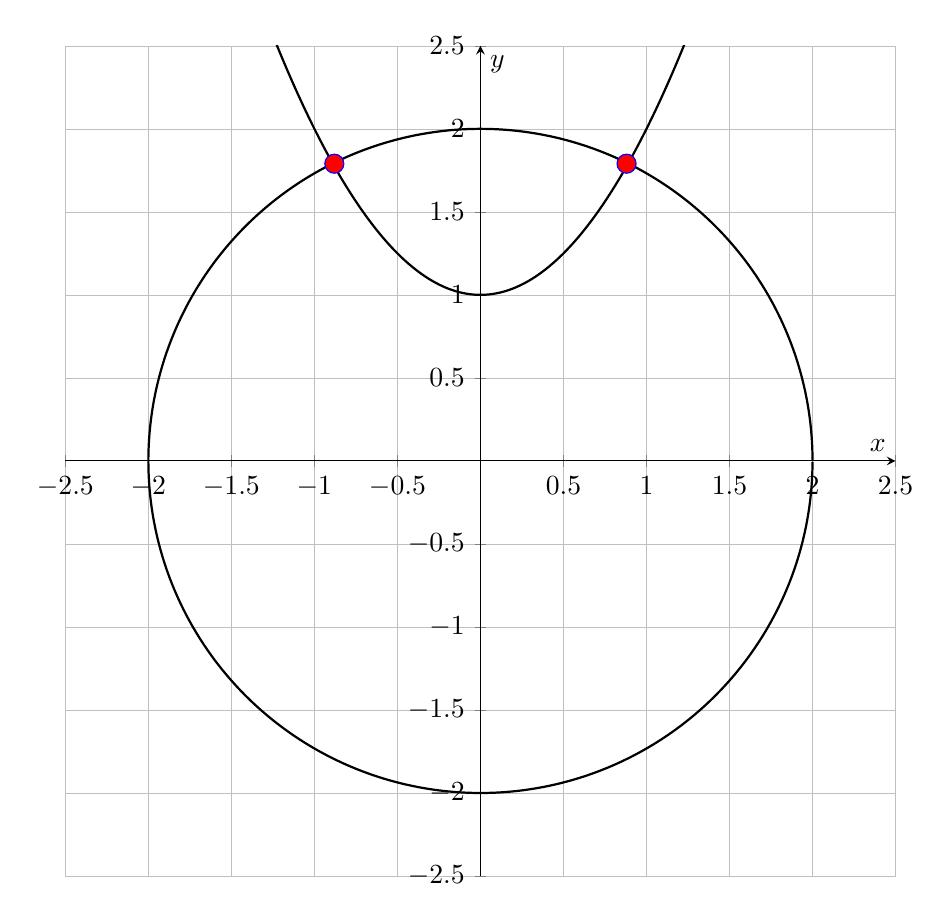
\begin{tikzpicture}
    \begin{axis}[
      axis lines=middle,
      xmin=-2.5,xmax=2.5,
      ymin=-2.5,ymax=2.5,
      xlabel={\(x\)},
      ylabel={\(y\)},
      grid=both,
      grid style={line width=.1pt, draw=gray!20},
      major grid style={line width=.2pt,draw=gray!50},
      width=\textwidth, height=\textwidth
    ]
    
    \coordinate (r0) at (0.88,1.79);
    \coordinate (r1) at (-0.88,1.79);
    
    
    % Draw the circle x^2 + y^2 = 4
    \addplot [samples=200, domain=0:2*3.14, smooth, thick] ({2*cos(deg(x))}, {2*sin(deg(x))});
    
    % Draw the parabola y = x^2 + 1
    \addplot [samples=200, domain=-2:2, smooth, thick] {x^2 + 1};
    
    \draw[fill=red, draw=blue] (r0) circle (0.01\textwidth);
    \draw[fill=red, draw=blue] (r1) circle (0.01\textwidth);
    
    \end{axis}
    \end{tikzpicture}
    \end{columns}
  \end{frame}
  
  \begin{frame}[fragile]
    \frametitle{Newton-Raphson Method: multi-dimensional case}
  
    \textbf{Extensions to multi-dimensional case:}
  
    \textbf{Check order of convergence:}
  
    \[
    \begin{array}{|c|c|c|c|c|c|c|}
    \hline
    \text{it} & x_1 & x_2 & \text{eps1} & \text{eps2} & m_1 & m_2 \\
    \hline
    1 & 1.0000 & 2.0000 & & & & \\
    2 & 0.9000 & 1.8000 & 0.1000 & 0.2000 & & \\
    3 & 0.8896 & 1.7913 & 0.0104 & 0.0087 & 1.9835 & 2.9482 \\
    4 & 0.8895 & 1.7913 & 0.0000699 & 0.0000165 & 2.0949 & 2.3208 \\
    5 & 0.8895 & 1.7913 & 0.0000000278 & 0.0000000059 & 2.0589 & 2.1382 \\
    \hline
    \end{array}
    \]
    
    \begin{block}{Quadratic convergence}
    Doubling number of significant digits every iteration
    \end{block}
    \[
    m = \frac{\ln(\varepsilon_{n+1}) - \ln(\varepsilon_n)}{\ln(\varepsilon_n) - \ln(\varepsilon_{n-1})}
    \]
  \end{frame}

  \begin{frame}[fragile]
    \frametitle{Newton-Raphson Method}
    
    \textbf{Deriving the extension to more than two variables}:
    \begin{columns}
      \begin{column}{0.5\textwidth}
        \begin{enumerate}
          \item Generalization to the N-dimensional case
          \item Define variables
          \item Multi-variate Taylor series expansion
          \item Define Jacobian matrix
          \item Neglect higher-order terms
          \item Express in terms of iterations
        \end{enumerate}
      \end{column}
      \begin{column}{0.5\textwidth}
        \begin{enumerate}
          \item 
            \( f_i(x_1, x_2, \ldots, x_N) = 0 \)
          \item 
            \( \mathbf{x} = [x_1, x_2, \ldots, x_N] \)
            \( \mathbf{f} = [f_1, f_2, \ldots, f_N] \)
          \item 
            \( f_i(\mathbf{x} + \delta \mathbf{x}) = f_i(\mathbf{x}) + \sum_{j=1}^{N} \frac{\partial f_i}{\partial x_j} \delta x_j + O(\delta \mathbf{x}^2) \)
          \item 
            \( J_{ij} = \frac{\partial f_i}{\partial x_j} \)
            \( f(\mathbf{x} + \delta \mathbf{x}) = f(\mathbf{x}) + \mathbf{J} \delta \mathbf{x} + O(\delta \mathbf{x}^2) \)
          \item 
            \( \mathbf{J} \cdot \delta \mathbf{x} = -\mathbf{f}(\mathbf{x}) \)
        \end{enumerate}
      \end{column}
    \end{columns}
    \[
      \boxed{\mathbf{x}_{n+1} = \mathbf{x}_n-\mathbf{J}^{-1}(\mathbf{x}_n)\cdot\mathbf{f}(\mathbf{x}_n)}
    \]
  \end{frame}
  
  
  \begin{frame}[fragile]
    \frametitle{Newton-Raphson Method}
    
    Multi-variate Newton-Raphson in Python:
    \begin{columns}
      \column{0.5\textwidth}
      \begin{lstlisting}[language=Python, basicstyle=\tiny]
def my_equations(X):
    F = np.zeros(2)
    F[0] = X[0]**2 + X[1]**2 - 4
    F[1] = X[0]**2 - X[1] + 1
    return F
      \end{lstlisting}
      \column{0.5\textwidth}
      \begin{lstlisting}[language=Python, basicstyle=\tiny]
def my_jac(x):
    jac = np.zeros((2, 2))
    jac[0, 0] = 2 * x[0]
    jac[0, 1] = 2 * x[1]
    jac[1, 0] = 2 * x[0]
    jac[1, 1] = -1
    return jac
      \end{lstlisting}
    \end{columns}
    \begin{lstlisting}[language=Python, basicstyle=\tiny]
import numpy as np
def newton_nd(f, J, x0, tol, max_iter):
    x = np.array(x0)
    err = np.zeros(max_iter)
    p = np.zeros(max_iter)
    for i in range(max_iter):
        delta_x = -np.linalg.solve(J(x), f(x))
        x += delta_x
        err[i] = np.linalg.norm(delta_x)
        if i > 0:
            p[i] = np.log(err[i]) / np.log(err[i-1])
        else:
            p[i] = float('nan')
        print(f'i = {i}: x = {x}, err = {err[i]:.6e}, p = {p[i]:.6f}')
        if err[i] < tol:
            break
    return x
    \end{lstlisting}
    \begin{lstlisting}[language=Python]
newton_nd(my_equations, my_jac, [1, 2], 1e-12, 100)
    \end{lstlisting}
\end{frame}


  \begin{frame}[fragile]
    \frametitle{Newton-Raphson Method}
  
    \textbf{Multi-variate Newton-Raphson in Python:}
    
    Plotting the functions:
    \begin{lstlisting}[language=Python]
plot_implicit_function(lambda x,y: y-x**2, resolution=100, colors="blue")
plot_implicit_function(lambda x,y: y**2+x**2-4, resolution=100, colors="red")
    \end{lstlisting}
    \begin{columns}
      \column{0.5\textwidth}
      \includegraphics[width=\textwidth]{circle_and_parabola_python.pdf}
      \column{0.5\textwidth}
      \begin{itemize}
        \item Code can be found in \lstinline[language=Python]{plot_implicit.py}
        \item Uses contour plot at $f(x,y)=0$
      \end{itemize}
      % \lstinputlisting[language=Python, basicstyle=\tiny]{scripts/nonlinear/plot_implicit.py}
    \end{columns}
  \end{frame}

  
\begin{frame}[fragile]
  \frametitle{Newton-Raphson Method}

  \textbf{Multi-variate Newton-Raphson in Python:}
  
  Plotting the norm of the function:
  \begin{lstlisting}[language=Python]
plot_surface_function(lambda x,y: np.sqrt((x**2 + y**2 -4)**2+(x**2-y+1)**2),
                         (0,3),(0,3))
        \end{lstlisting}
        \begin{columns}
          \column{0.5\textwidth}
          \includegraphics[width=0.8\textwidth]{surface_circ_par_error.pdf}
          \column{0.5\textwidth}
          \begin{itemize}
            \item Code can be found in \lstinline[language=Python]{plot_implicit.py}
            \item Uses contour plot at $f(x,y)=0$
          \end{itemize}
          % \lstinputlisting[language=Python, basicstyle=\tiny]{scripts/nonlinear/plot_implicit.py}
        \end{columns}
\end{frame}

\begin{frame}[fragile]
  \frametitle{Newton-Raphson Method}

  \textbf{Multi-variate Newton-Raphson in Python:}
  
  Plotting the norm of the function:
  \begin{lstlisting}[language=Python]
plot_contours(lambda x,y: np.sqrt((x**2 + y**2 -4)**2+(x**2-y+1)**2),
                 (0, 3), (0, 3), resolution = 100, levels=[0, 1, 2, 3, 4])
        \end{lstlisting}
        \begin{columns}
          \column{0.5\textwidth}
          \includegraphics[width=0.8\textwidth]{surface_circ_par_error_contour.pdf}
          \column{0.5\textwidth}
          \begin{itemize}
            \item Code can be found in \lstinline[language=Python]{plot_implicit.py}
            \item Uses contour plot at $f(x,y)=0$
          \end{itemize}
          % \lstinputlisting[language=Python, basicstyle=\tiny]{scripts/nonlinear/plot_implicit.py}
        \end{columns}
\end{frame}

  \begin{frame}[fragile]
    \frametitle{Broyden's Method}
    
    \textbf{Multi-dimensional secant method ('quasi-Newton'):}
    \begin{itemize}
      \item Disadvantage of the Newton-Raphson method:
        \begin{itemize}
          \item It requires the Jacobian matrix.
          \item In many problems, no analytical Jacobian is available.
          \item If the function evaluation is expensive, the numerical approximation using finite differences can be prohibitive.
        \end{itemize}
      \item Solution: Use a cheap approximation of the Jacobian! (Secant or 'quasi-Newton' method)
      \item Comparison:
        \[
        \text{Newton-Raphson:} \quad J_{ij}(\mathbf{x}) = \frac{\partial f_i}{\partial x_j}(\mathbf{x}) \quad \text{(Analytical)}
        \]
        \[
        \text{Secant method:} \quad \mathbf{J}(\mathbf{x}) \quad \text{approximated by}\quad \mathbf{B} \quad \text{(Numerical)}
        \]
    \end{itemize}
  \end{frame}

  \begin{frame}[fragile]
    \frametitle{Broyden's Method}
  
    \textbf{Approximating $\mathbf{B}^{n+1}$:}
    \begin{itemize}
      \item Multi-dimensional secant method ('quasi-Newton'):
      \item Secant equation (generalization of 1D case):
      \[
        \mathbf{B}^{n+1} \cdot \delta \mathbf{x}^n=\delta \mathbf{f}^n \quad \delta \mathbf{x}^n=\mathbf{x}^{n+1}-\mathbf{x}^n \quad \delta \mathbf{f}^n=\mathbf{f}^{n+1}-\mathbf{f}^n
      \]
      \item Underdetermined (not unique: -n equations with n unknowns), need another condition to pin down \(B^{n+1}\).
    \end{itemize}
    \textbf{Broyden's method:}
    \begin{itemize}
      \item  Determine \(\mathbf{B}^{n+1}\) by making the least change to \(\mathbf{B}^{n}\) that is consistent with the secant condition.
      \item Updating formula:
      \[
        \mathbf{B}^{n+1}=\mathbf{B}^n+\frac{\left(\delta \mathbf{f}^n-\mathbf{B}^n \cdot \delta \mathbf{x}^n\right)}{\delta \mathbf{x}^n \cdot \delta \mathbf{x}^n} \otimes \delta \mathbf{x}^n
      \]
      \item Note: Sometimes \(\delta B_{n-1}\) is updated directly.
    \end{itemize}
  \end{frame}
  
  \begin{frame}[fragile]
    \frametitle{Broyden's Method}
  
    \textbf{Background of Broyden’s method:}
    \begin{itemize}
      \item Secant equation:
      \[
      \textbf{B}^{n+1} \cdot \delta \textbf{x}^n = \delta f_{n}
      \]
      \item Since there is no update on derivative info, why would \(\textbf{B}^{n}\) change in a direction orthogonal to \(\delta \textbf{x}^n\)?
      \[
        \Rightarrow (\delta \textbf{x}^n)^T \delta \textbf{w} = 0
      \]
      % \item Updating formula:
      \vspace{-0.5cm}
      \begin{columns}
        \column{0.1\textwidth}
        \column{0.2\textwidth}
        \begin{align*}
          &\textbf{B}^{n+1}\cdot\textbf{w} = \textbf{B}^{n}\cdot\textbf{w}\\
          &\textbf{B}^{n+1}\cdot\delta \textbf{x}^n = \delta \textbf{f}^n
        \end{align*}
        \column{0.05\textwidth}
        \[
          \Rightarrow  
        \]
        \column{0.65\textwidth}
        \[
          \mathbf{B}^{n+1}=\mathbf{B}^n+\frac{\left(\delta \mathbf{f}^n-\mathbf{B}^n \cdot \delta \mathbf{x}^n\right)}{\delta \mathbf{x}^n \cdot \delta \mathbf{x}^n} \otimes \delta \mathbf{x}^n
        \]
      \end{columns}
      \vspace{0.5cm}
      \item Initialize \(\delta \textbf{x}^n\) and \(\textbf{B}_{0}\) with the identity matrix (or with finite difference approx.).
    \end{itemize}
  \end{frame}


  \begin{frame}[fragile]
    \frametitle{Broyden's Method}
    \textbf{Python implementation of Broyden's method:}
    \begin{columns}
      \column{0.5\textwidth}
    \begin{itemize}
      \item Same example as before but now with Broyden's method.
      \item Slower convergence with Broyden's method should be offset by improved efficiency of each iteration!
      \begin{lstlisting}[language=Python]
broyden(@MyFunc,[1;2],1e-12,1e-12)
      \end{lstlisting}
      \item Requires 11 iterations (compare with Newton: 5 iterations)
      
      But much fewer function evaluations per iteration!
    \end{itemize}
  
    \column{0.5\textwidth}
    \begin{lstlisting}[language=Python]
import numpy as np
from numpy.linalg import inv

def broyden(F, x0, tol=1e-6, max_iter=100):
    x = np.array(x0)
    B = np.eye(x.size)
    for i in range(max_iter):
        Fx = F(x)
        if np.linalg.norm(Fx) < tol:
            print(f"Converged after {i} iterations.")
            return x
        x_new = x - inv(B)@Fx
        delta_x = x_new - x
        delta_Fx = F(x_new) - Fx
        B += np.outer((delta_Fx - B@delta_x)/(delta_x@delta_x), delta_x)
        x = x_new
    print("Max iterations reached.")
    return x
    \end{lstlisting}
  \end{columns}
  \end{frame}

  
  \begin{frame}[fragile]
    \frametitle{Broyden's Method}
  
    \begin{itemize}
      \item Same example as before but now with Broyden's method.
      \item Note how the approximate Jacobian (\(\textbf{B}\)) is updated over subsequent iterations:
      
      \begin{tiny}
        \begin{align*}
          \begin{bmatrix}
          1. & 0. \\
          0. & 1.
          \end{bmatrix} & \rightarrow &
          \begin{bmatrix}
          3. & -1. \\
          4. & -1.
          \end{bmatrix} & \rightarrow &
          \begin{bmatrix}
          -1.0 & -9.0 \\
          3.4 & -2.2
          \end{bmatrix} & \rightarrow &
          \begin{bmatrix}
          -1.062 & -9.260 \\
          3.411 & -2.154
          \end{bmatrix} & \rightarrow &\\
          \begin{bmatrix}
          5.290 & -3.864 \\
          2.493 & -2.934
          \end{bmatrix} & \rightarrow &
          \begin{bmatrix}
          7.363 & -1.931 \\
          3.556 & -1.943
          \end{bmatrix} & \rightarrow &
          \begin{bmatrix}
          2.349 & -0.773 \\
          3.547 & -1.941
          \end{bmatrix} & \rightarrow &
          \begin{bmatrix}
          -0.934 & -6.772 \\
          2.351 & -4.124
          \end{bmatrix} & \rightarrow &\\
          \begin{bmatrix}
          -0.384 & -5.879 \\
          2.500 & -3.884
          \end{bmatrix} & \rightarrow &
          \begin{bmatrix}
          10.416 & 6.344 \\
          5.947 & 0.018
          \end{bmatrix} & \rightarrow &
          \begin{bmatrix}
          9.781 & 5.515 \\
          5.641 & -0.382
          \end{bmatrix} & \rightarrow &
          \begin{bmatrix}
          3.577 & 3.630 \\
          3.362 & -1.074
          \end{bmatrix} & \rightarrow &\\
          \begin{bmatrix}
          3.116 & 3.238 \\
          2.912 & -1.458
          \end{bmatrix} & \rightarrow &
          \begin{bmatrix}
          1.992 & 3.272 \\
          1.989 & -1.430
          \end{bmatrix} & \rightarrow & \hdots & \rightarrow & \hdots & \rightarrow &
  \end{align*}  
    \end{tiny}

    \item Compare with analytical jacobian:
    \(
      \textbf{B}=\begin{bmatrix}
      1.748 & 3.261 \\
      1.736 & -1.439
      \end{bmatrix}\quad
      \textbf{J}=
      \begin{bmatrix}
      1.779 & 3.583 \\
      1.779 & -1
      \end{bmatrix}
      \)
      \item Note that the approximate Jacobian (\(\textbf{B}\)) is not exact even when the solution has already been found!
    \end{itemize}
  \end{frame}
  
  \begin{frame}[fragile]
    \frametitle{Conclusions}
  
    \begin{itemize}
      \item Recommendations for root finding:
      \begin{itemize}
        \item One-dimensional cases:
        \begin{itemize}
          \item If it is not easy/cheap to compute the function's derivative $\Rightarrow$ use Brent's algorithm.
          \item If derivative information is available $\Rightarrow$ use Newton-Raphson's method + bookkeeping on bounds provided you can supply a good enough initial guess!!
          \item There are specialized routines for (multiple) root finding of polynomials (but not covered in this course).
        \end{itemize}
        \item Multi-dimensional cases:
        \begin{itemize}
          \item Use Newton-Raphson method, but make sure that you provide an initial guess close enough to achieve convergence.
          \item In case derivative information is expensive $\Rightarrow$ use Broyden's method (but slower convergence!).
        \end{itemize}
      \end{itemize}
    \end{itemize}
  \end{frame}
  
  